\documentclass[12pt]{article}
\usepackage{graphicx}
\usepackage{amsmath}
\usepackage{placeins}

\begin{document}

\begin{titlepage}
    \begin{center}
        \huge
        FIR Filter Design\\Using Kaiser Window
        \vfill
        \large
        Student Details:\\\vspace{3pt}
        Name: Kanak Yadav\\\vspace{3pt}
        Roll No: 20D070044\\\vspace{3pt}
        Filter Number: 55\\\vspace{3pt}
        Group Number: 37\\\vspace{60pt}
        Reviewer Details:\\\vspace{3pt}
        Name: Pal Abhijeet Manoj\\\vspace{3pt}
        Roll No: 200100107
        \vfill
    \end{center}
\end{titlepage}

\section{Bandpass Filter Design}
\subsection{Un-normalized Discrete Time Filter}
\hline
\vspace{10pt}
\textbf{Specifications:}
\begin{itemize}
    \item Passband: 100 kHz to 175 kHz,
    \item Stopband: 0 to 95 kHz and 180 kHz to 300 kHz (since $f_s$ = 600 kHz),
    \item Passband and Stopband tolerance: 0.15,
    \item Passband and Stopband nature: we do not have a choice of nature.
\end{itemize}
\hline

\subsection{Normalized Digital Filter}

\begin{table}[h]
    \centering
    \begin{tabular}{|c|c|}\hline
         Discrete-time frequency&Normalized digital frequency\\
         $f$ (kHz)&$\omega$ (radians)\\\hline
         0&0\\\hline
         95&$\omega_{s1}$ = 0.9948377\\\hline
         100&$\omega_{p1}$ = 1.0471976\\\hline
         175&$\omega_{p2}$ = 1.8325957\\\hline
         180&$\omega_{s2}$ = 1.8849556\\\hline
         300&$\pi$\\\hline
    \end{tabular}
    \caption{Normalizing frequency.}
    \label{tab:1}
\end{table}
\newline
\hline
\vspace{10pt}
\textbf{Specifications:}
\begin{itemize}
    \item Passband: 1.0471976 to 1.8325957,
    \item Stopband: 0 to 0.9948377 and 1.8849556 to  $\pi$,
    \item Passband and Stopband tolerance: 0.15,
    \item Passband and Stopband nature: we do not have a choice of nature.
\end{itemize}
\hline

\newpage
\subsection{$\text{h}_\text{ideal}[\text{n}]$}
The ideal impulse response of the bandpass filter with the specifications can be made by using two ideal low-pass filters having cut-off frequencies in the middle of the transition band:
\begin{align*}
    \omega_{c1} &= \frac{\omega_{s1} + \omega_{p1}}{2} = 1.0210176,\\
    \omega_{c2} &= \frac{\omega_{p2} + \omega_{s2}}{2} = 1.8587757.
\end{align*}
\[\text{h}_\text{ideal}[\text{n}] = sinc(\omega_{c2}.n)\frac{\omega_{c2}}{\pi} - sinc(\omega_{c1}.n)\frac{\omega_{c1}}{\pi}\]

\subsection{Kaiser window}
\[A = -20.\log_{10}(\delta) = -20.\log_{10}(0.15) = 16.478175.\]
\begin{align*}
    \alpha &= 0.1102(A-8.7) \, for A > 50\\
    &= 0.5842(A-21)^{0.4} + 0.07886(A-21) \, for \, 50 \geq A \geq 21\\
    &= 0 \, for \, 20 > A
\end{align*}
hence,\[\alpha = 0.\]
\[\beta = \frac{\alpha}{N} = 0.\]
For $\beta = 0$,\[I_o(\beta) = 1.\]
Thus, the kaiser window function is simply the rectangular window function from -N to +N.\[v[k] = \frac{I_o\left(\beta N\sqrt{1-(\frac{k}{N})^2}\right)}{I_o(\beta N)} = 1; \,\, k \, \epsilon \, [-N, +N]\]
Choosing N:
\begin{align*}
    2N + 1 &\ge 1 + \frac{A - 8}{2.285\Delta\omega_T}\\
    \Delta\omega_T = \omega_{s1} - \omega_{p1} &= \omega_{p2} - \omega_{s2} = 0.0523599\\
    2N + 1 &\ge 71.862675\\
    N &\ge 35.4313375
\end{align*}
Since N should be a positive integer,\[N \ge 36.\]
\subsection{Filter Transfer Function}
For the exact value of N, we must evaluate whether the magnitude tolerances at the transition band edges are satisfied. For this, we would have to iterate over N and find the magnitude of the FIR filter transfer function at the passband and stopband edges. Shifting the response for causality,
\[\text{h}_\text{fir}[\text{n + N}] = \text{h}_\text{ideal}[\text{n}].\text{v}[\text{n}],\]
\[\text{H}_\text{fir}[\text{z}] = \sum_{n = 0}^{2N}\text{h}_\text{fir}[\text{n}]\text{z}^{-n}.\]
Note that the window length is 2N + 1 for a given N. The smallest value of N that satisfies all the requirements of the Bandpass filter is:\[N = 46.\]
\begin{center}
    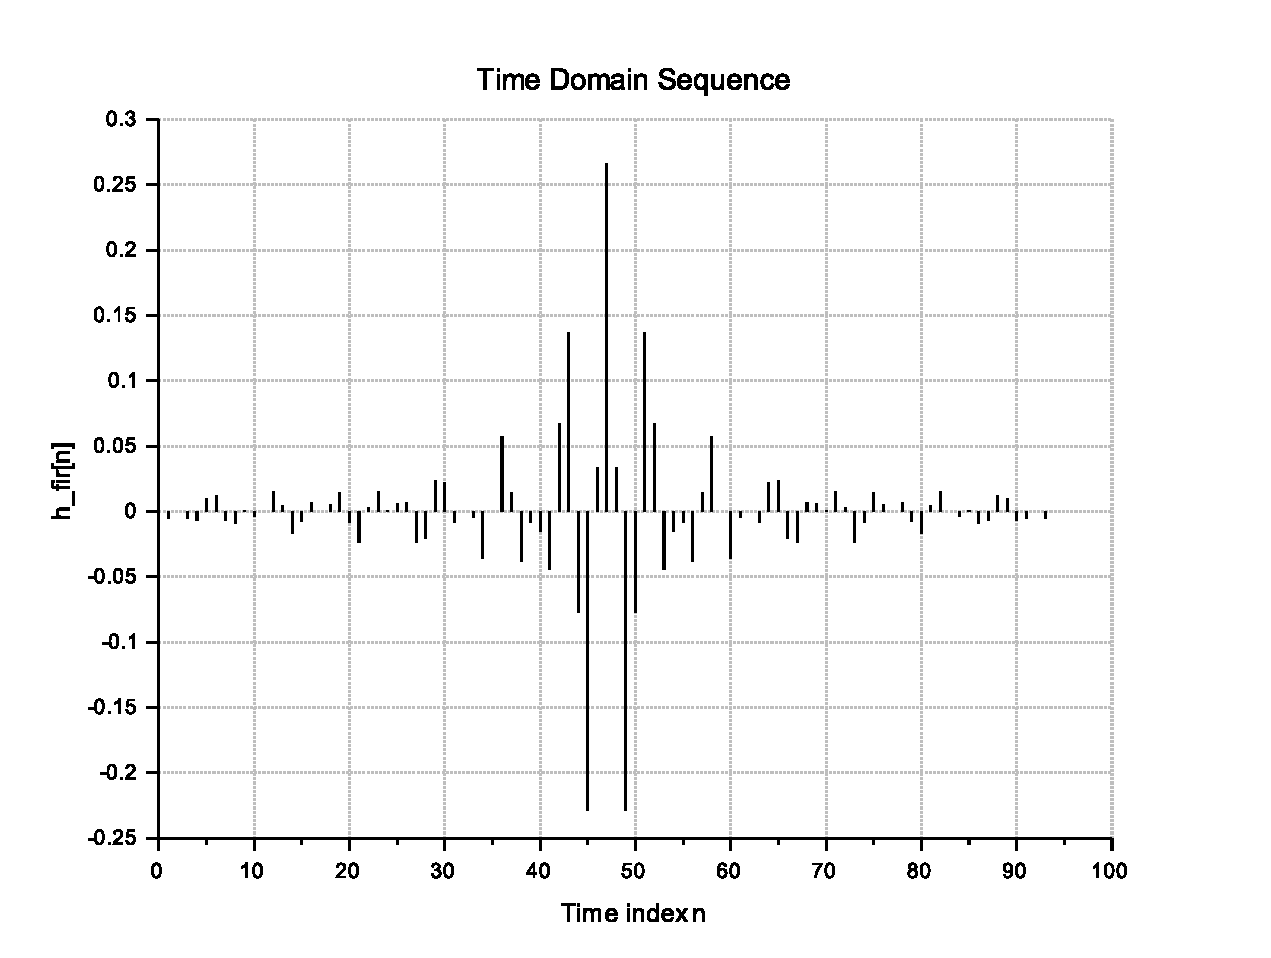
\includegraphics[width=\textwidth]{time_bp.pdf}
\end{center}
\begin{center}
    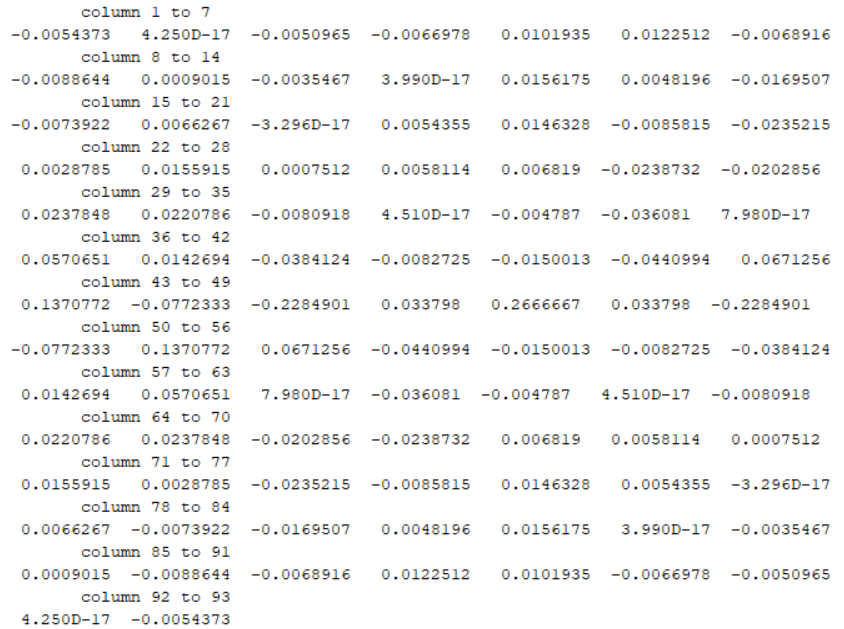
\includegraphics[width=\textwidth]{h_fir_bp.png}
\end{center}
Time index n and column n in the above figures correspond to the coefficient of $\text{z}^{-\text{n}+1}$
\newpage
\subsection{Frequency Response}
\begin{center}
    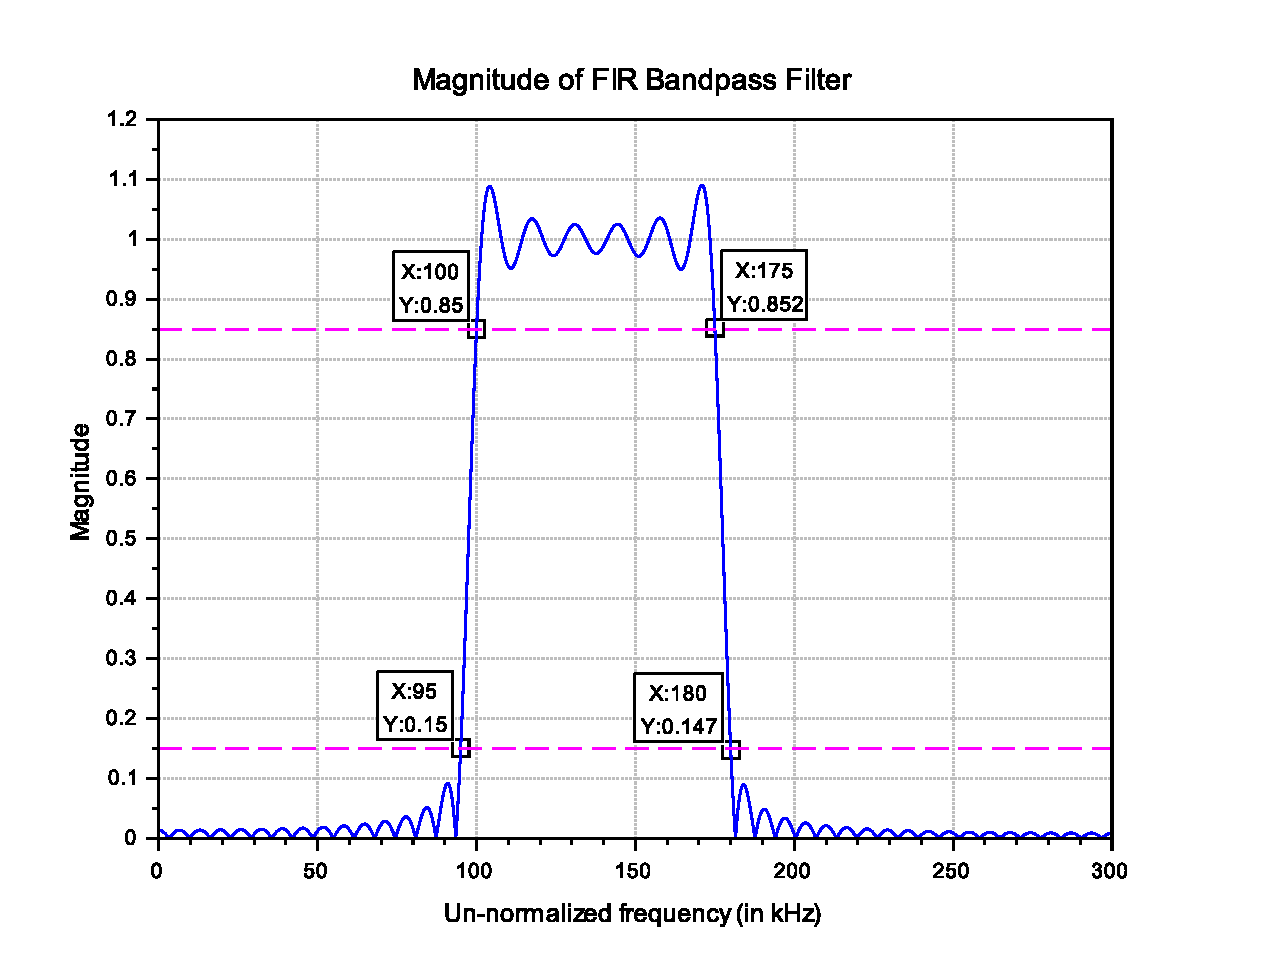
\includegraphics[scale=0.6]{mag_bp.pdf}
    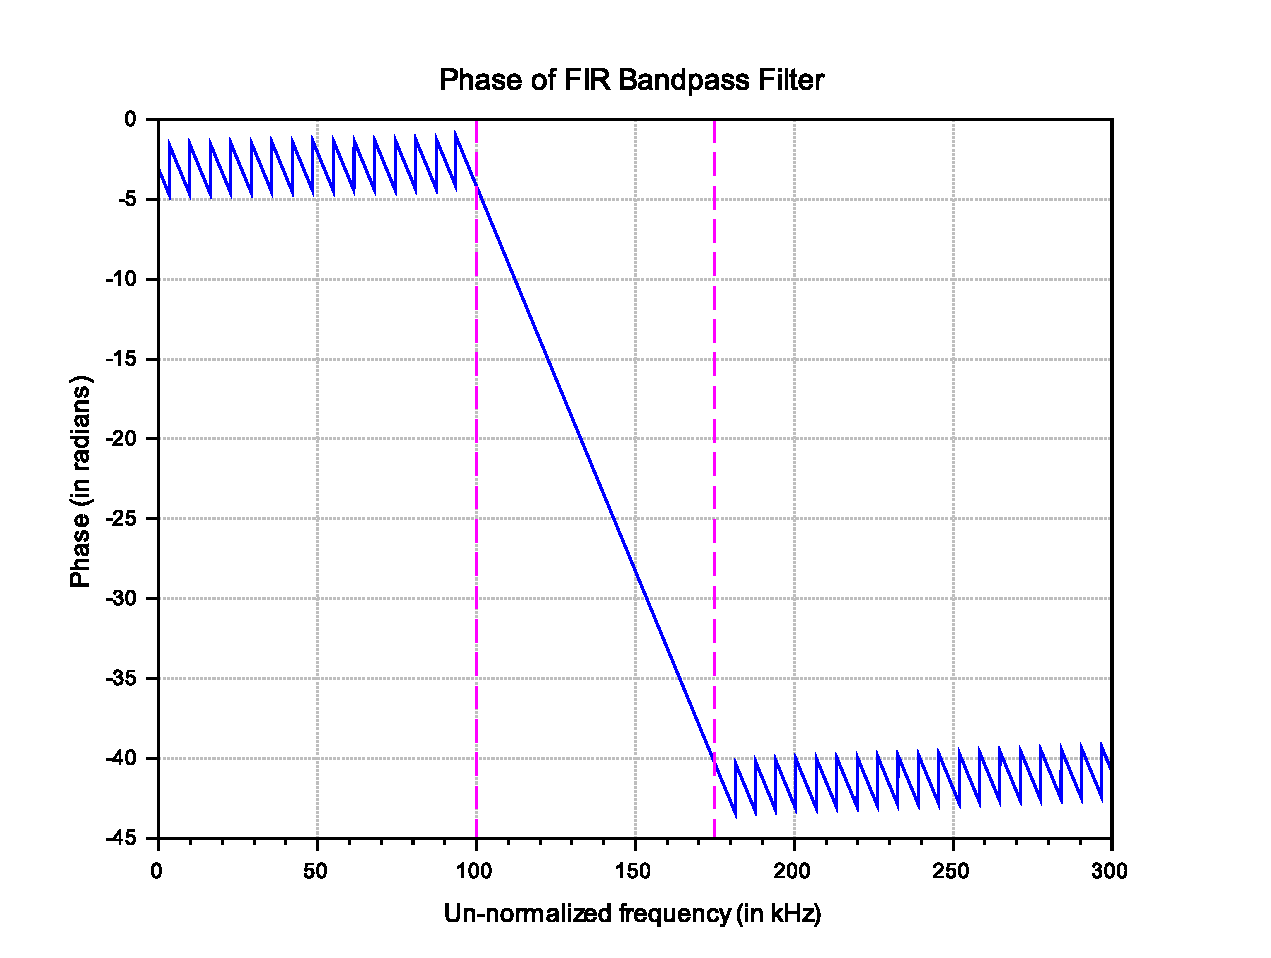
\includegraphics[scale=0.6]{phase_bp.pdf}
\end{center}

\section{Bandstop Filter Design}
\subsection{Un-normalized Discrete Time Filter}
\hline
\vspace{10pt}
\textbf{Specifications:}
\begin{itemize}
    \item Passband: 0 to 85 kHz and 135 kHz to 212.5 kHz (since $f_s$ = 425 kHz),
    \item Stopband: 90 kHz to 130 kHz,
    \item Passband and Stopband tolerance: 0.15,
    \item Passband and Stopband nature: we do not have a choice of nature.
\end{itemize}
\hline

\subsection{Normalized Digital Filter}

\begin{table}[h]
    \centering
    \begin{tabular}{|c|c|}\hline
         Discrete-time frequency&Normalized digital frequency\\
         $f$ (kHz)&$\omega$ (radians)\\\hline
         0&0\\\hline
         85&$\omega_{p1}$ = 1.2566371\\\hline
         90&$\omega_{s1}$ = 1.3305569\\\hline
         130&$\omega_{s2}$ = 1.9219155\\\hline
         135&$\omega_{p2}$ = 1.9958353\\\hline
         212.5&$\pi$\\\hline
    \end{tabular}
    \caption{Normalizing frequency.}
    \label{tab:1}
\end{table}
\newline
\hline
\vspace{10pt}
\textbf{Specifications:}
\begin{itemize}
    \item Passband: 0 to 1.2566371 and 1.9958353 to  $\pi$,
    \item Stopband: 1.3305569 to 1.9219155,
    \item Passband and Stopband tolerance: 0.15,
    \item Passband and Stopband nature: we do not have a choice of nature.
\end{itemize}
\hline

\newpage
\subsection{$\text{h}_\text{ideal}[\text{n}]$}
The ideal impulse response of the bandstop filter with the specifications can be made by using an all-pass filter and two ideal low-pass filters having cut-off frequencies in the middle of the transition band:
\begin{align*}
    \omega_{c1} &= \frac{\omega_{p1} + \omega_{s1}}{2} = 1.2935970,\\
    \omega_{c2} &= \frac{\omega_{s2} + \omega_{p2}}{2} = 1.9588754.
\end{align*}
\[\text{h}_\text{ideal}[\text{n}] = sinc(\pi.n) - sinc(\omega_{c2}.n)\frac{\omega_{c2}}{\pi} + sinc(\omega_{c1}.n)\frac{\omega_{c1}}{\pi}\]

\subsection{Kaiser window}
For the Bandstop filter, we again obtain the shape parameter $\beta$ = 0, hence a rectangular window with the bound on N being:\[N \ge 26.\]

\subsection{Filter Transfer Function}
For the exact value of N, we must evaluate whether the magnitude tolerances at the transition band edges are satisfied. For this, we would have to iterate over N and find the magnitude of the FIR filter transfer function at the passband and stopband edges. Shifting the response for causality,
\[\text{h}_\text{fir}[\text{n + N}] = \text{h}_\text{ideal}[\text{n}].\text{v}[\text{n}],\]
\[\text{H}_\text{fir}[\text{z}] = \sum_{n = 0}^{2N}\text{h}_\text{fir}[\text{n}]\text{z}^{-n}.\]
Note that the window length is 2N + 1 for a given N. The smallest value of N that satisfies all the requirements of the Bandpass filter is:\[N = 33.\]
\begin{center}
    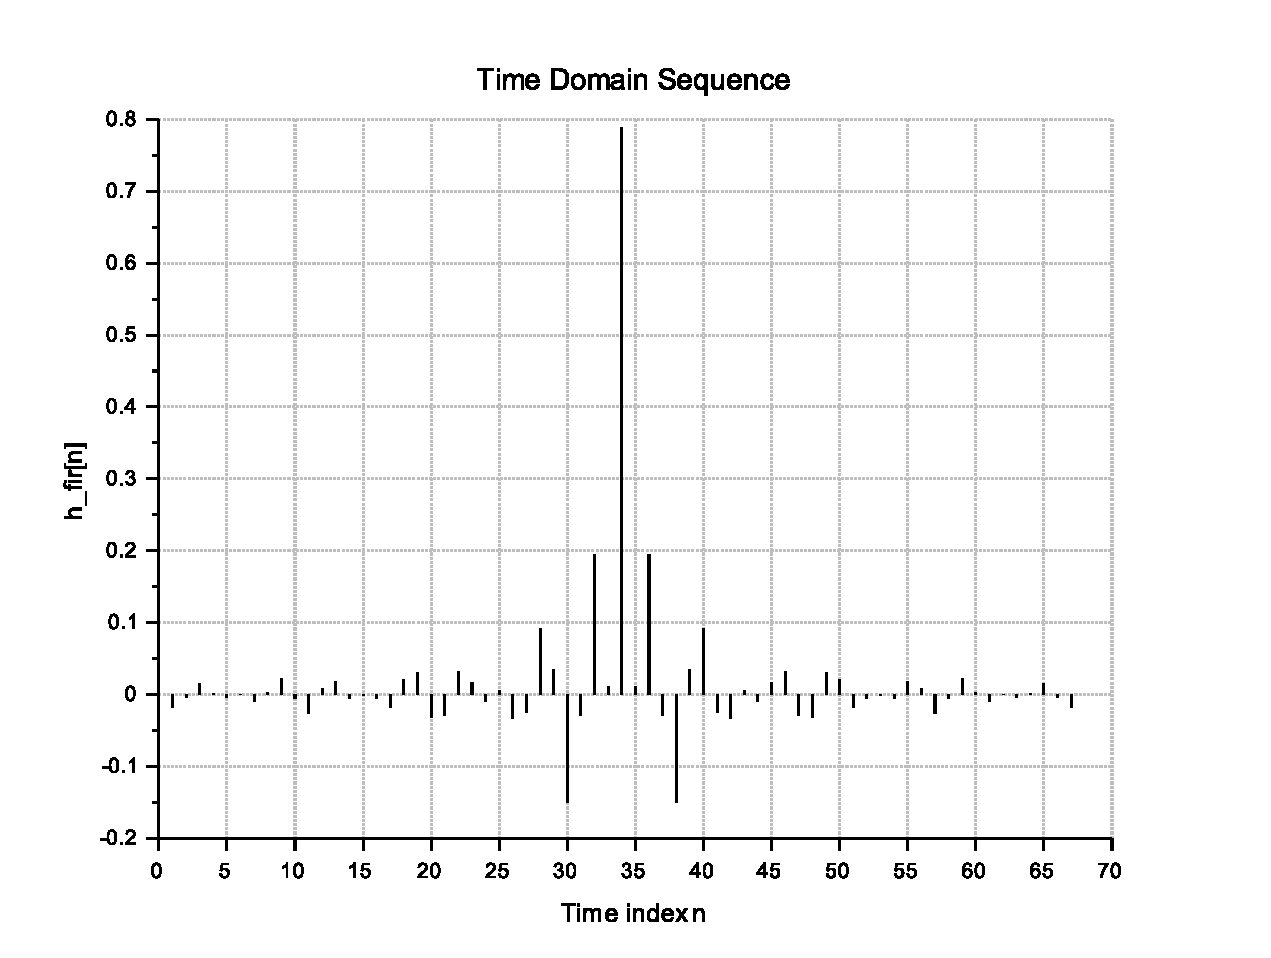
\includegraphics[width=\textwidth]{time_bs.pdf}
\end{center}
\begin{center}
    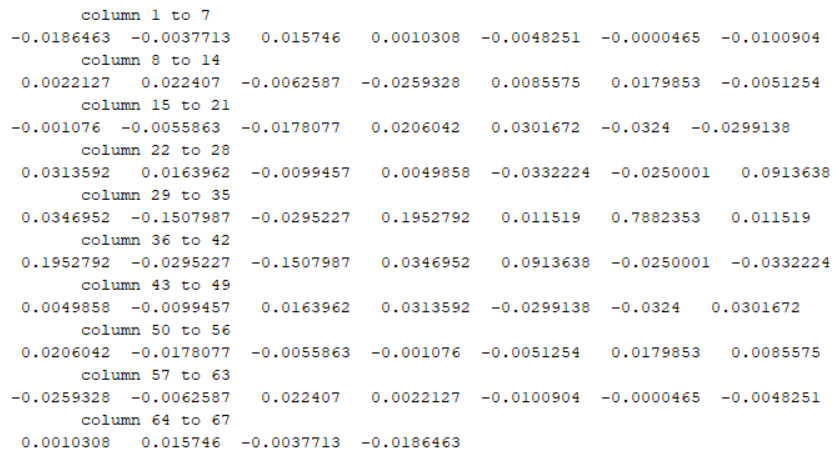
\includegraphics[width=\textwidth]{h_fir_bs.png}
\end{center}
Time index n and column n in the above figures correspond to the coefficient of $\text{z}^{-\text{n}+1}$

\subsection{Frequency Response}
\begin{center}
    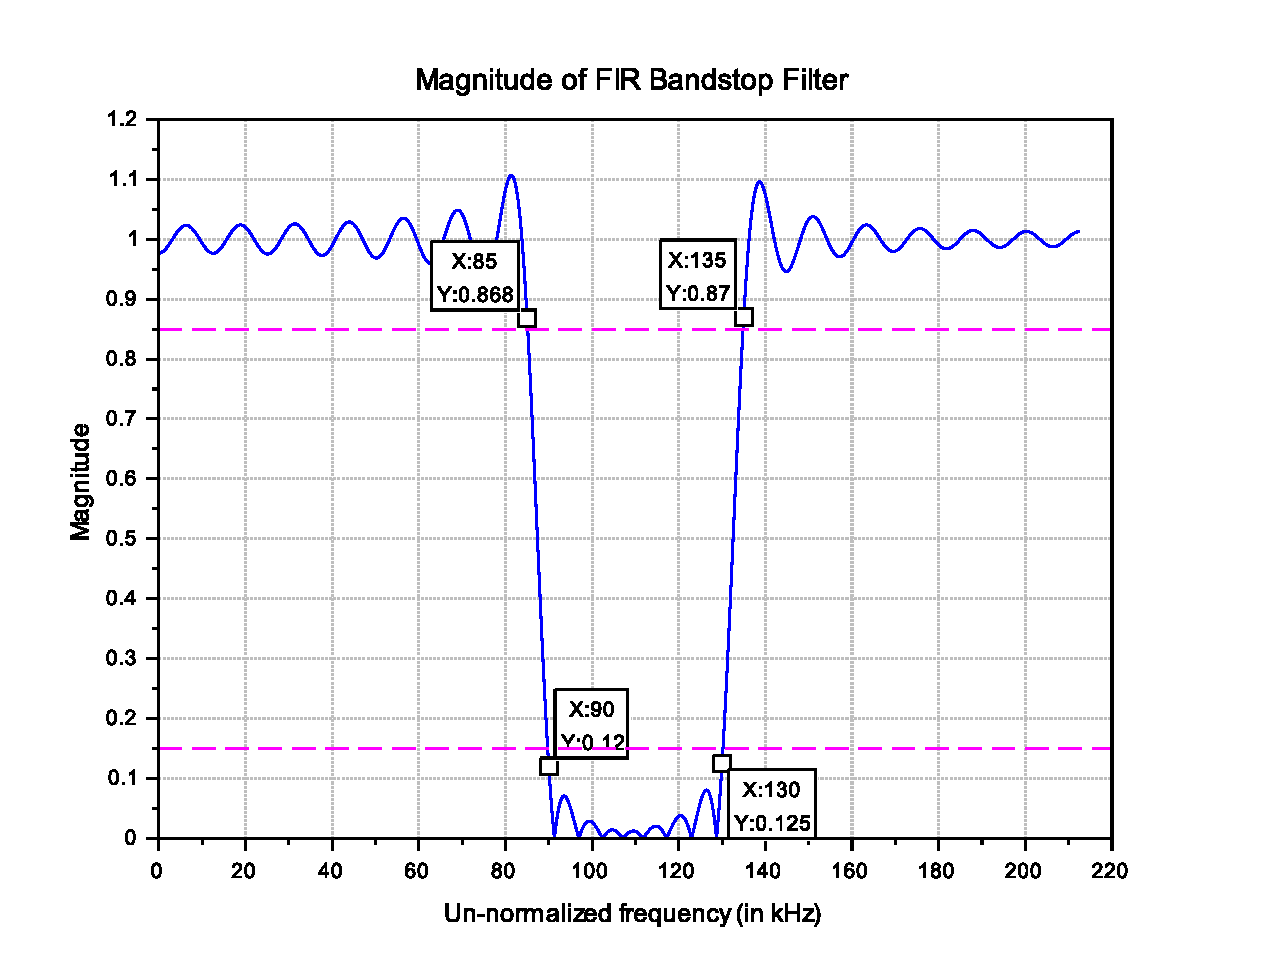
\includegraphics[scale=0.6]{mag_bs.pdf}
    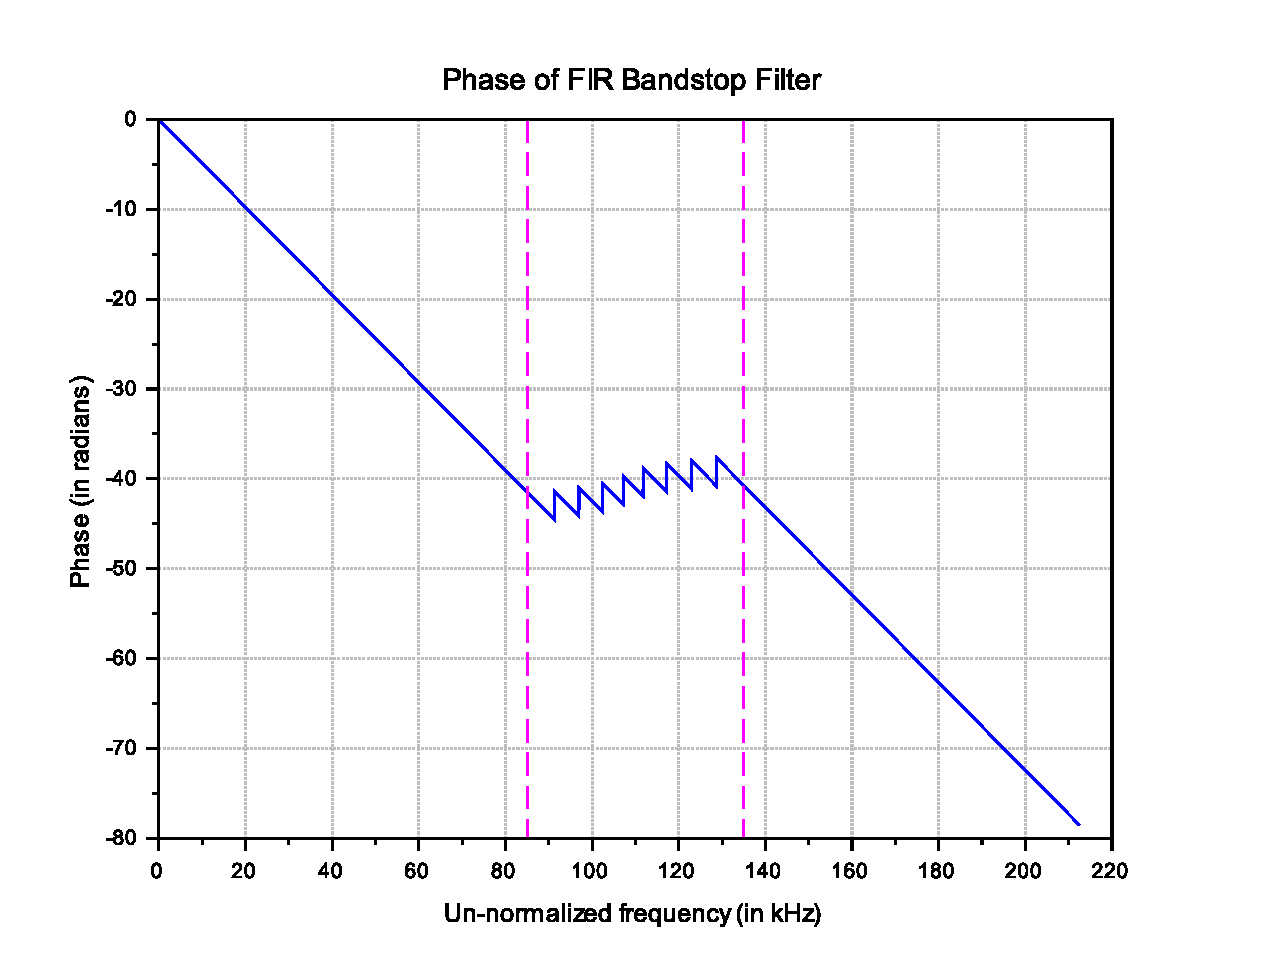
\includegraphics[scale=0.6]{phase_bs.pdf}
\end{center}

\section{Comparison with IIR realizations}
The plots comparing the responses of the IIR and FIR filters may be viewed from  the next page onwards.
\subsection{Magnitude Response}
The FIR filters have a sharper transition band than the IIR filters. However, the nature of the response in the passband and stopband is preferred in the following order: Constant $>$ Monotonic $>$ Equiripple. The FIR filter is unable to achieve either of these and gives a rippled response where the ripples converge toward the cut-off frequencies as we increase N (for the rectangular window) but their heights remain unchanged.
\subsection{Phase Response}
The adjustable phase response is the main advantage of the FIR filters and we observe that in the passband of both filters, the phase response is linear whereas that of the IIR filters is non-linear. Outside the pass band, however, the phase response shows a sawtooth-like pattern.

\section{Review}
I have reviewed Abhijeet's (200100107) report and certify it to be correct.

\begin{figure}[h!]
    \centering
    \noindent\makebox[width=\textwidth]{%
    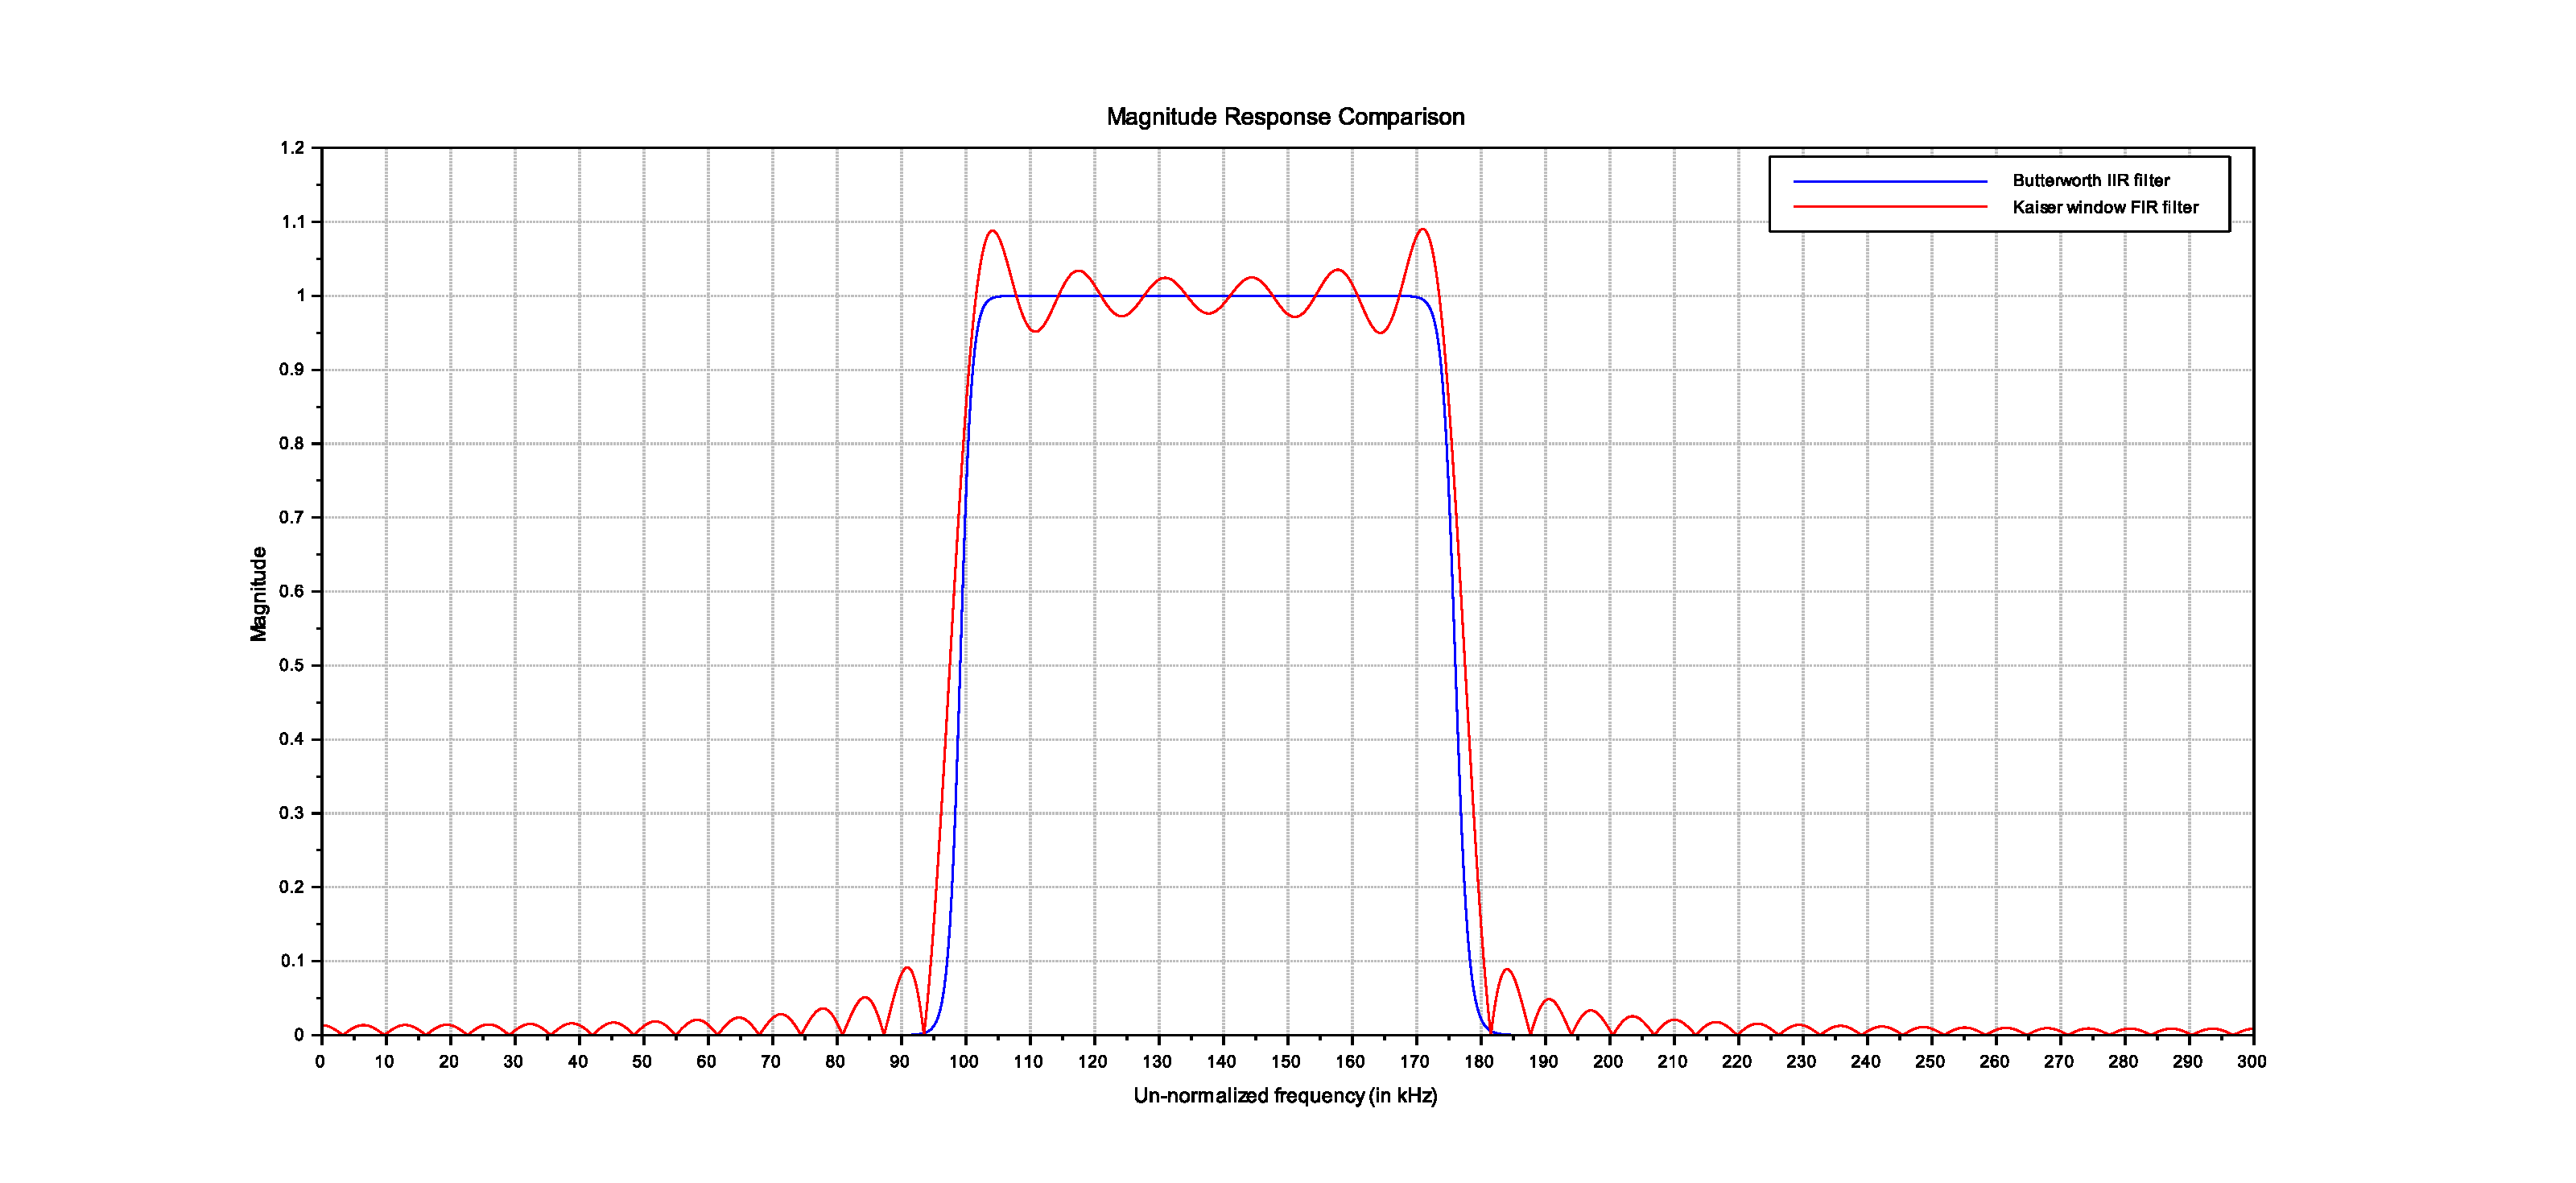
\includegraphics[width=1.5\textwidth]{comp_bp_mag.pdf}}
    \vfill
    \noindent\makebox[width=\textwidth]{%
    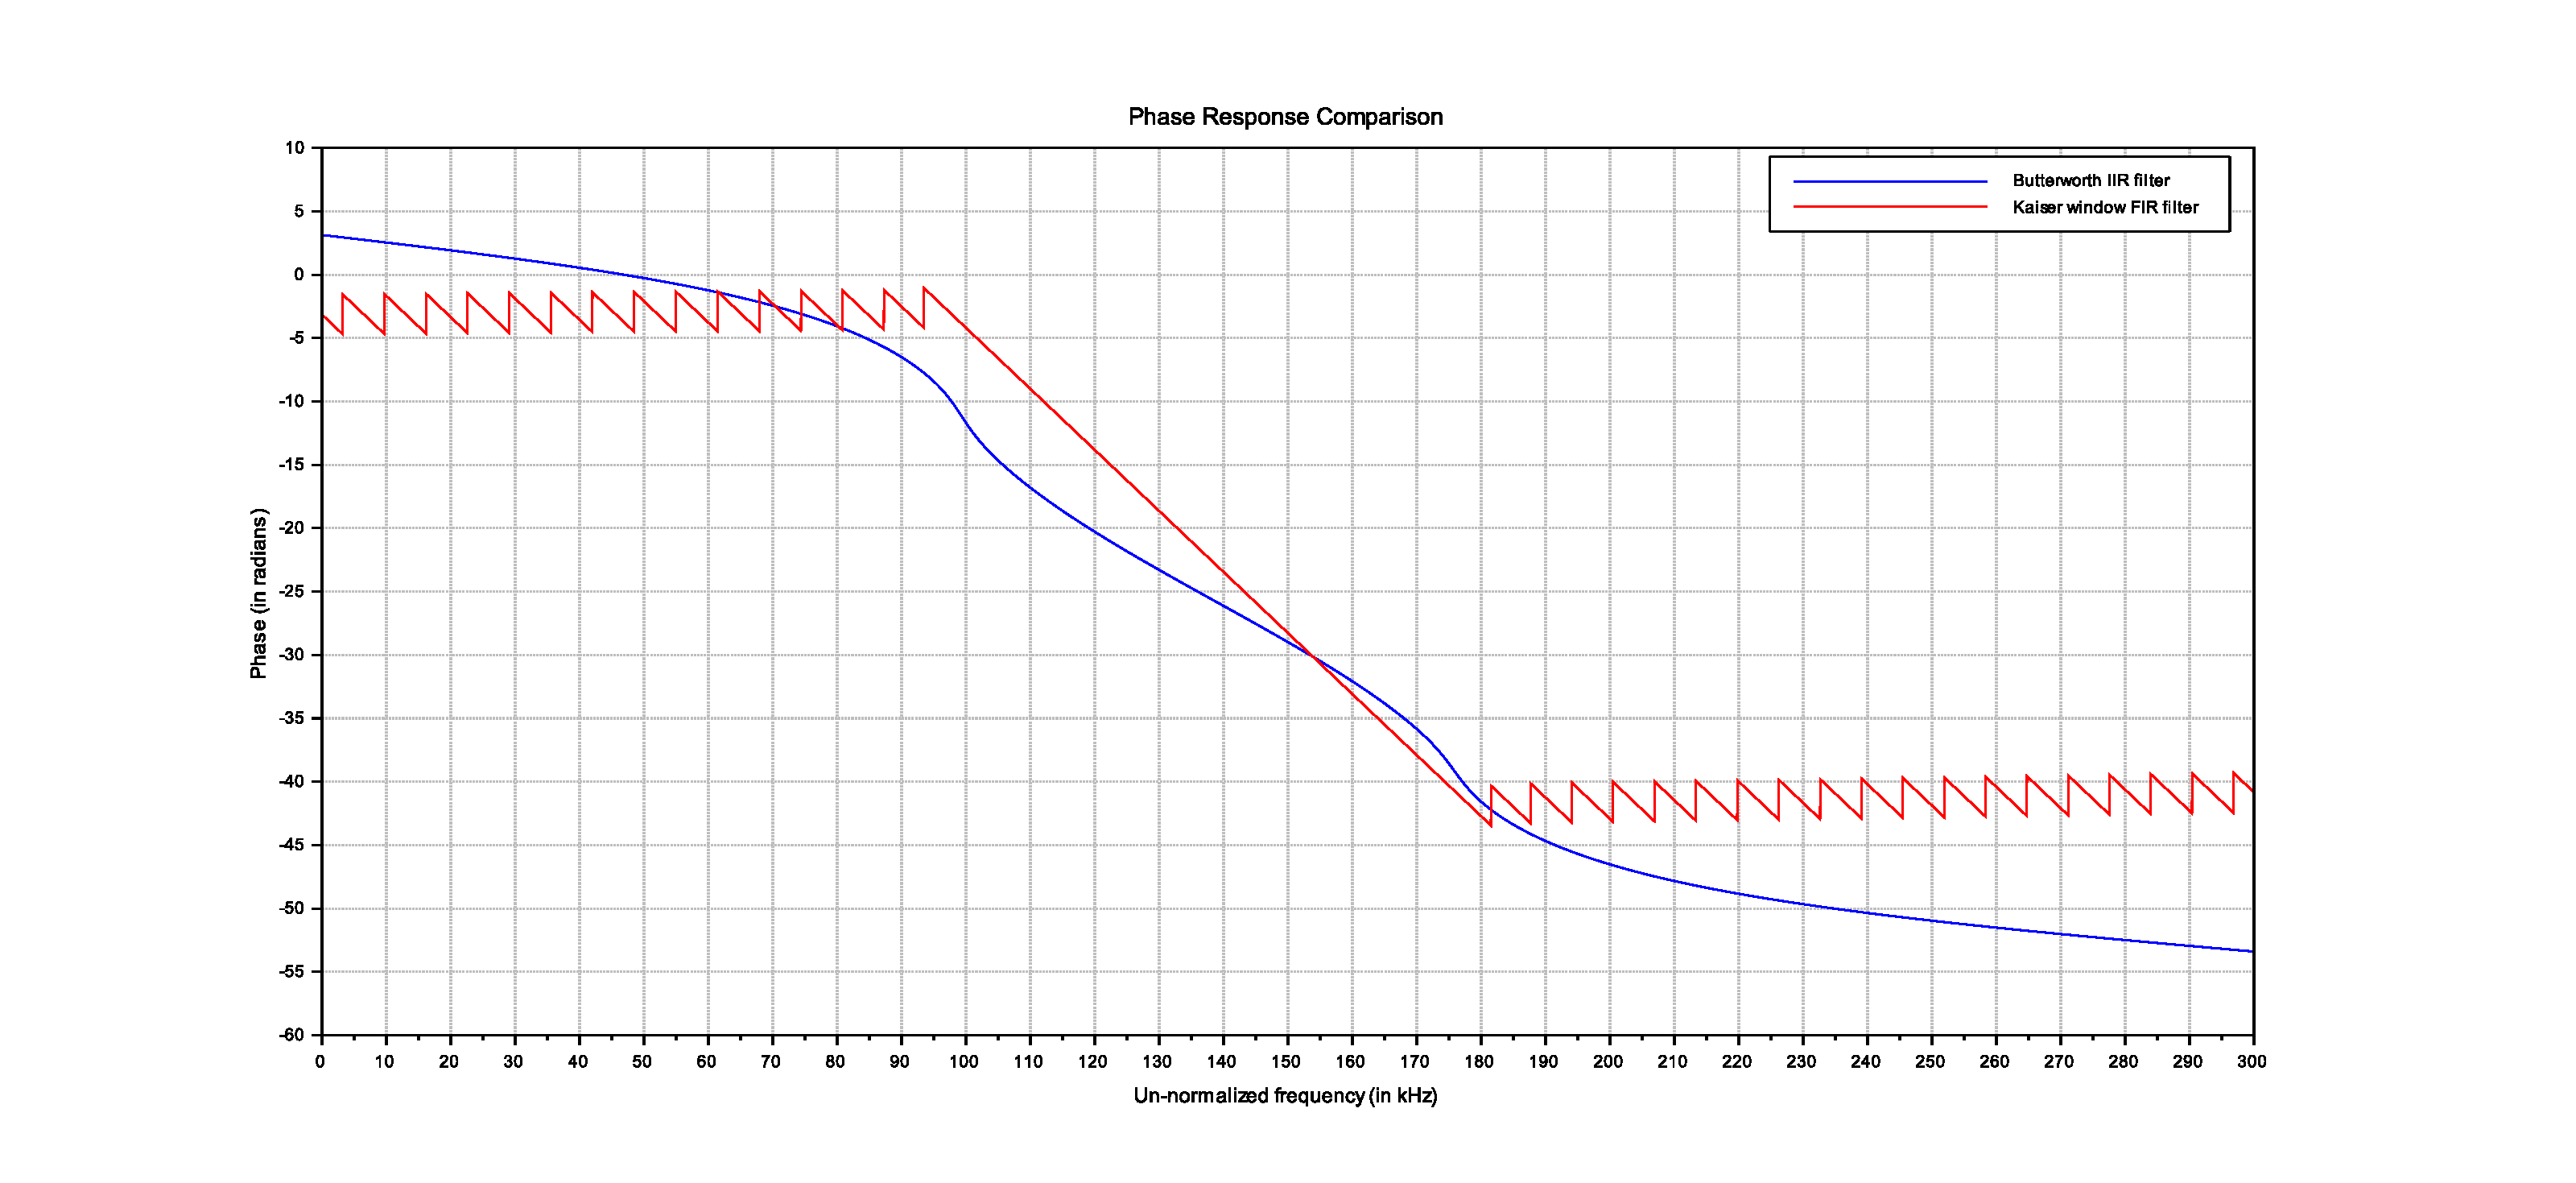
\includegraphics[width=1.5\textwidth]{comp_bp_phase.pdf}}
\end{figure}
\begin{figure}[h!]
    \centering
    \noindent\makebox[width=\textwidth]{%
    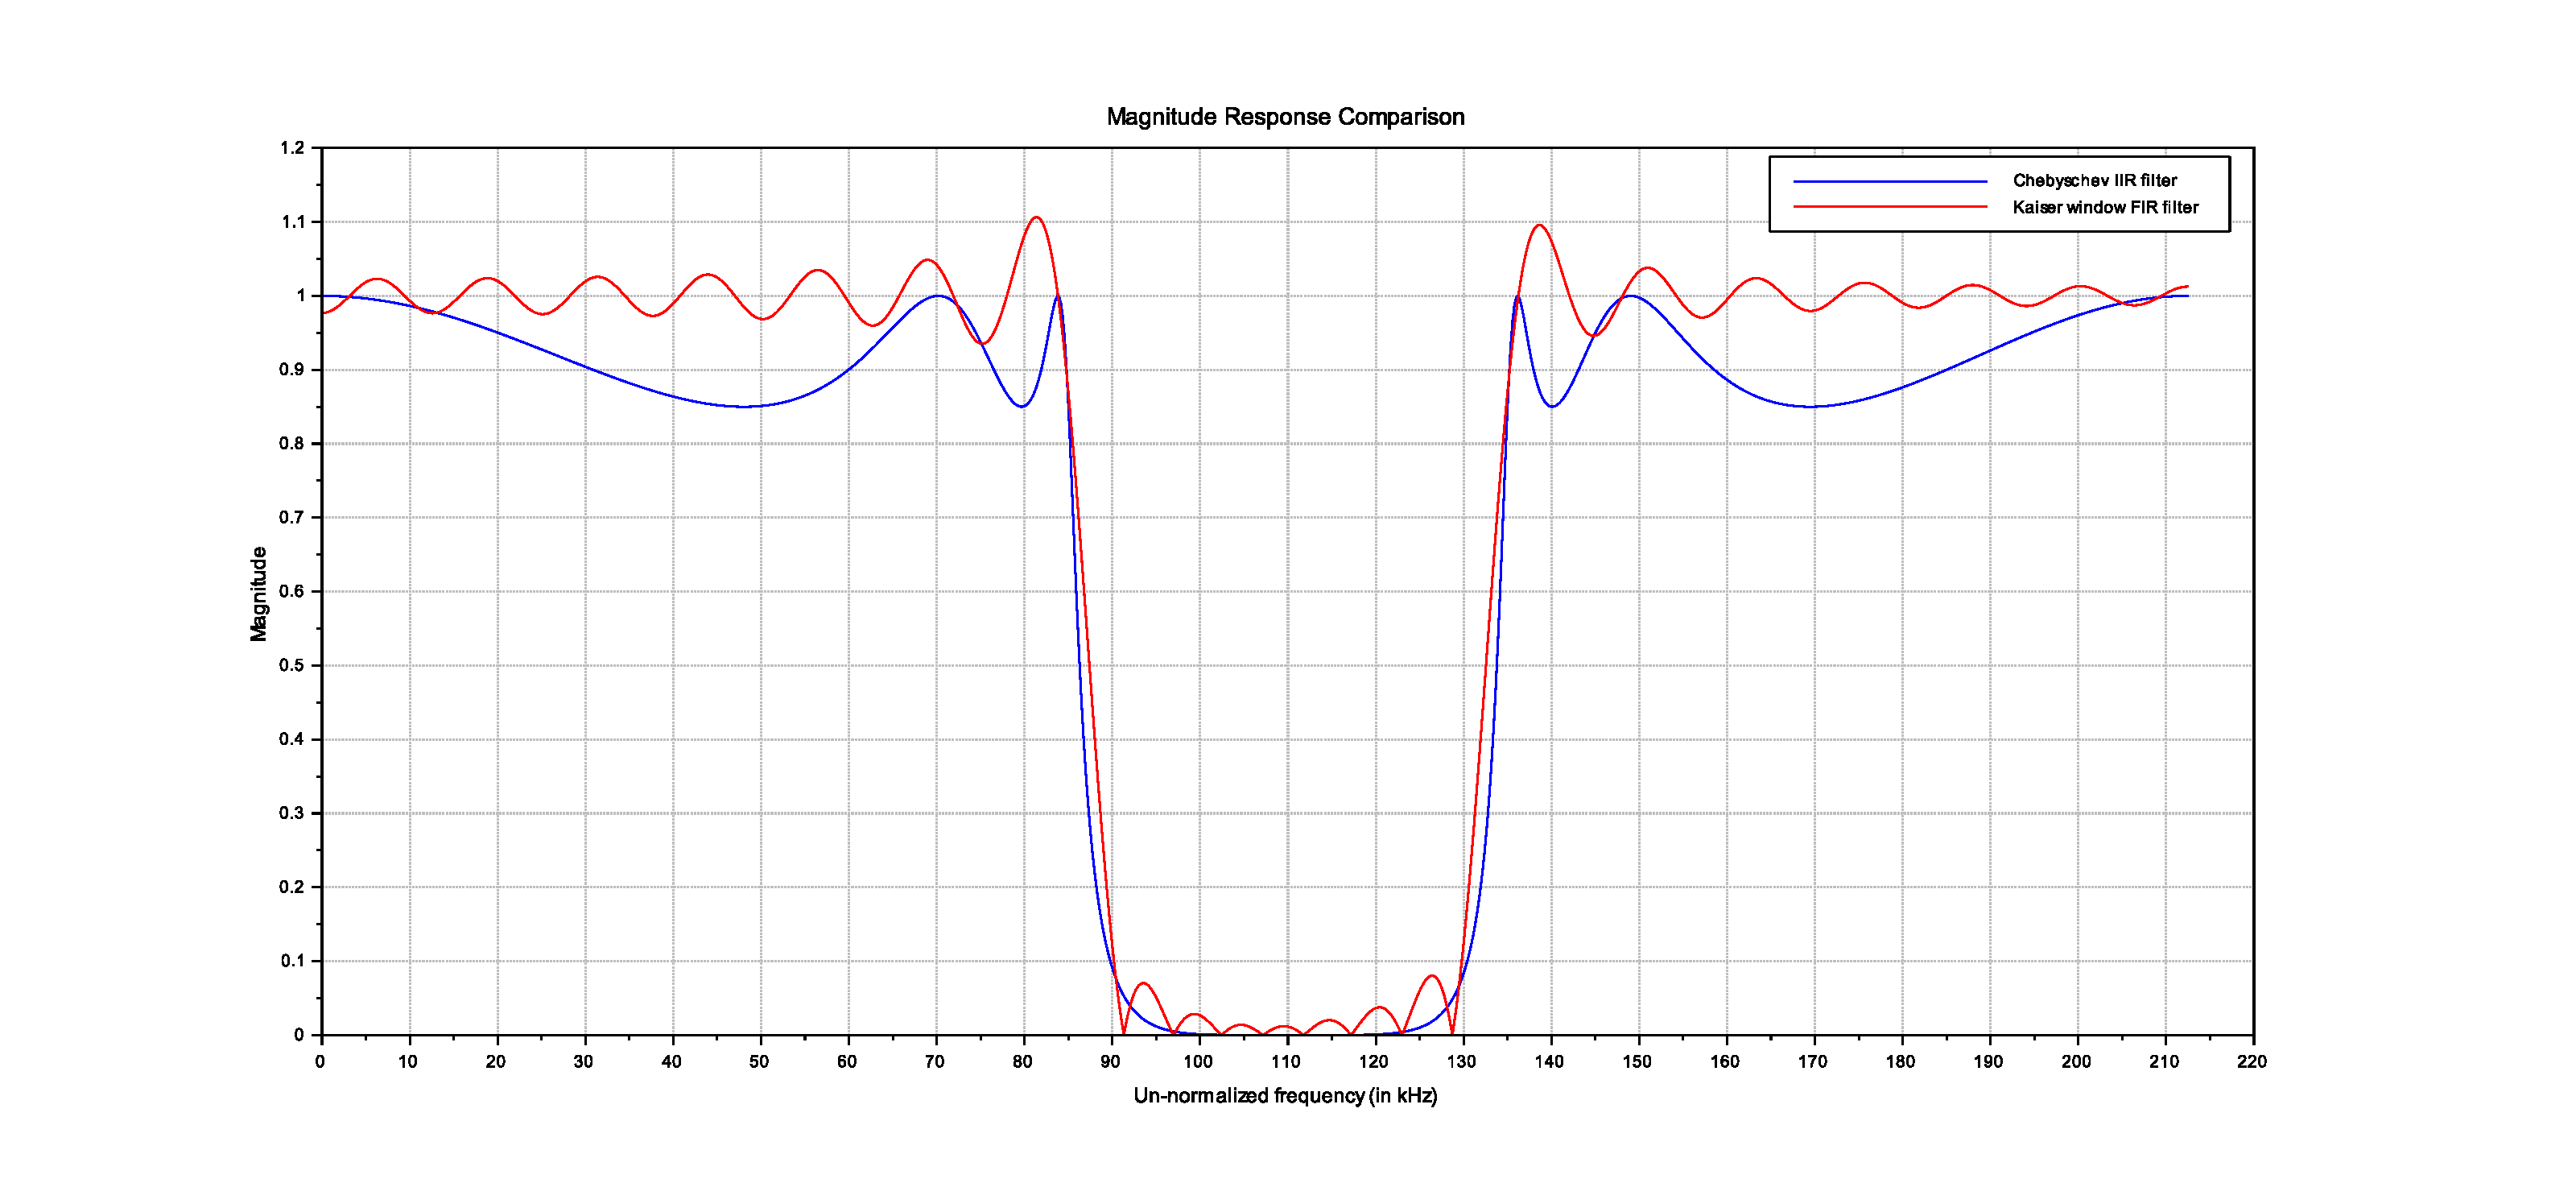
\includegraphics[width=1.5\textwidth]{comp_bs_mag.pdf}}
    \vfill
    \noindent\makebox[width=\textwidth]{%
    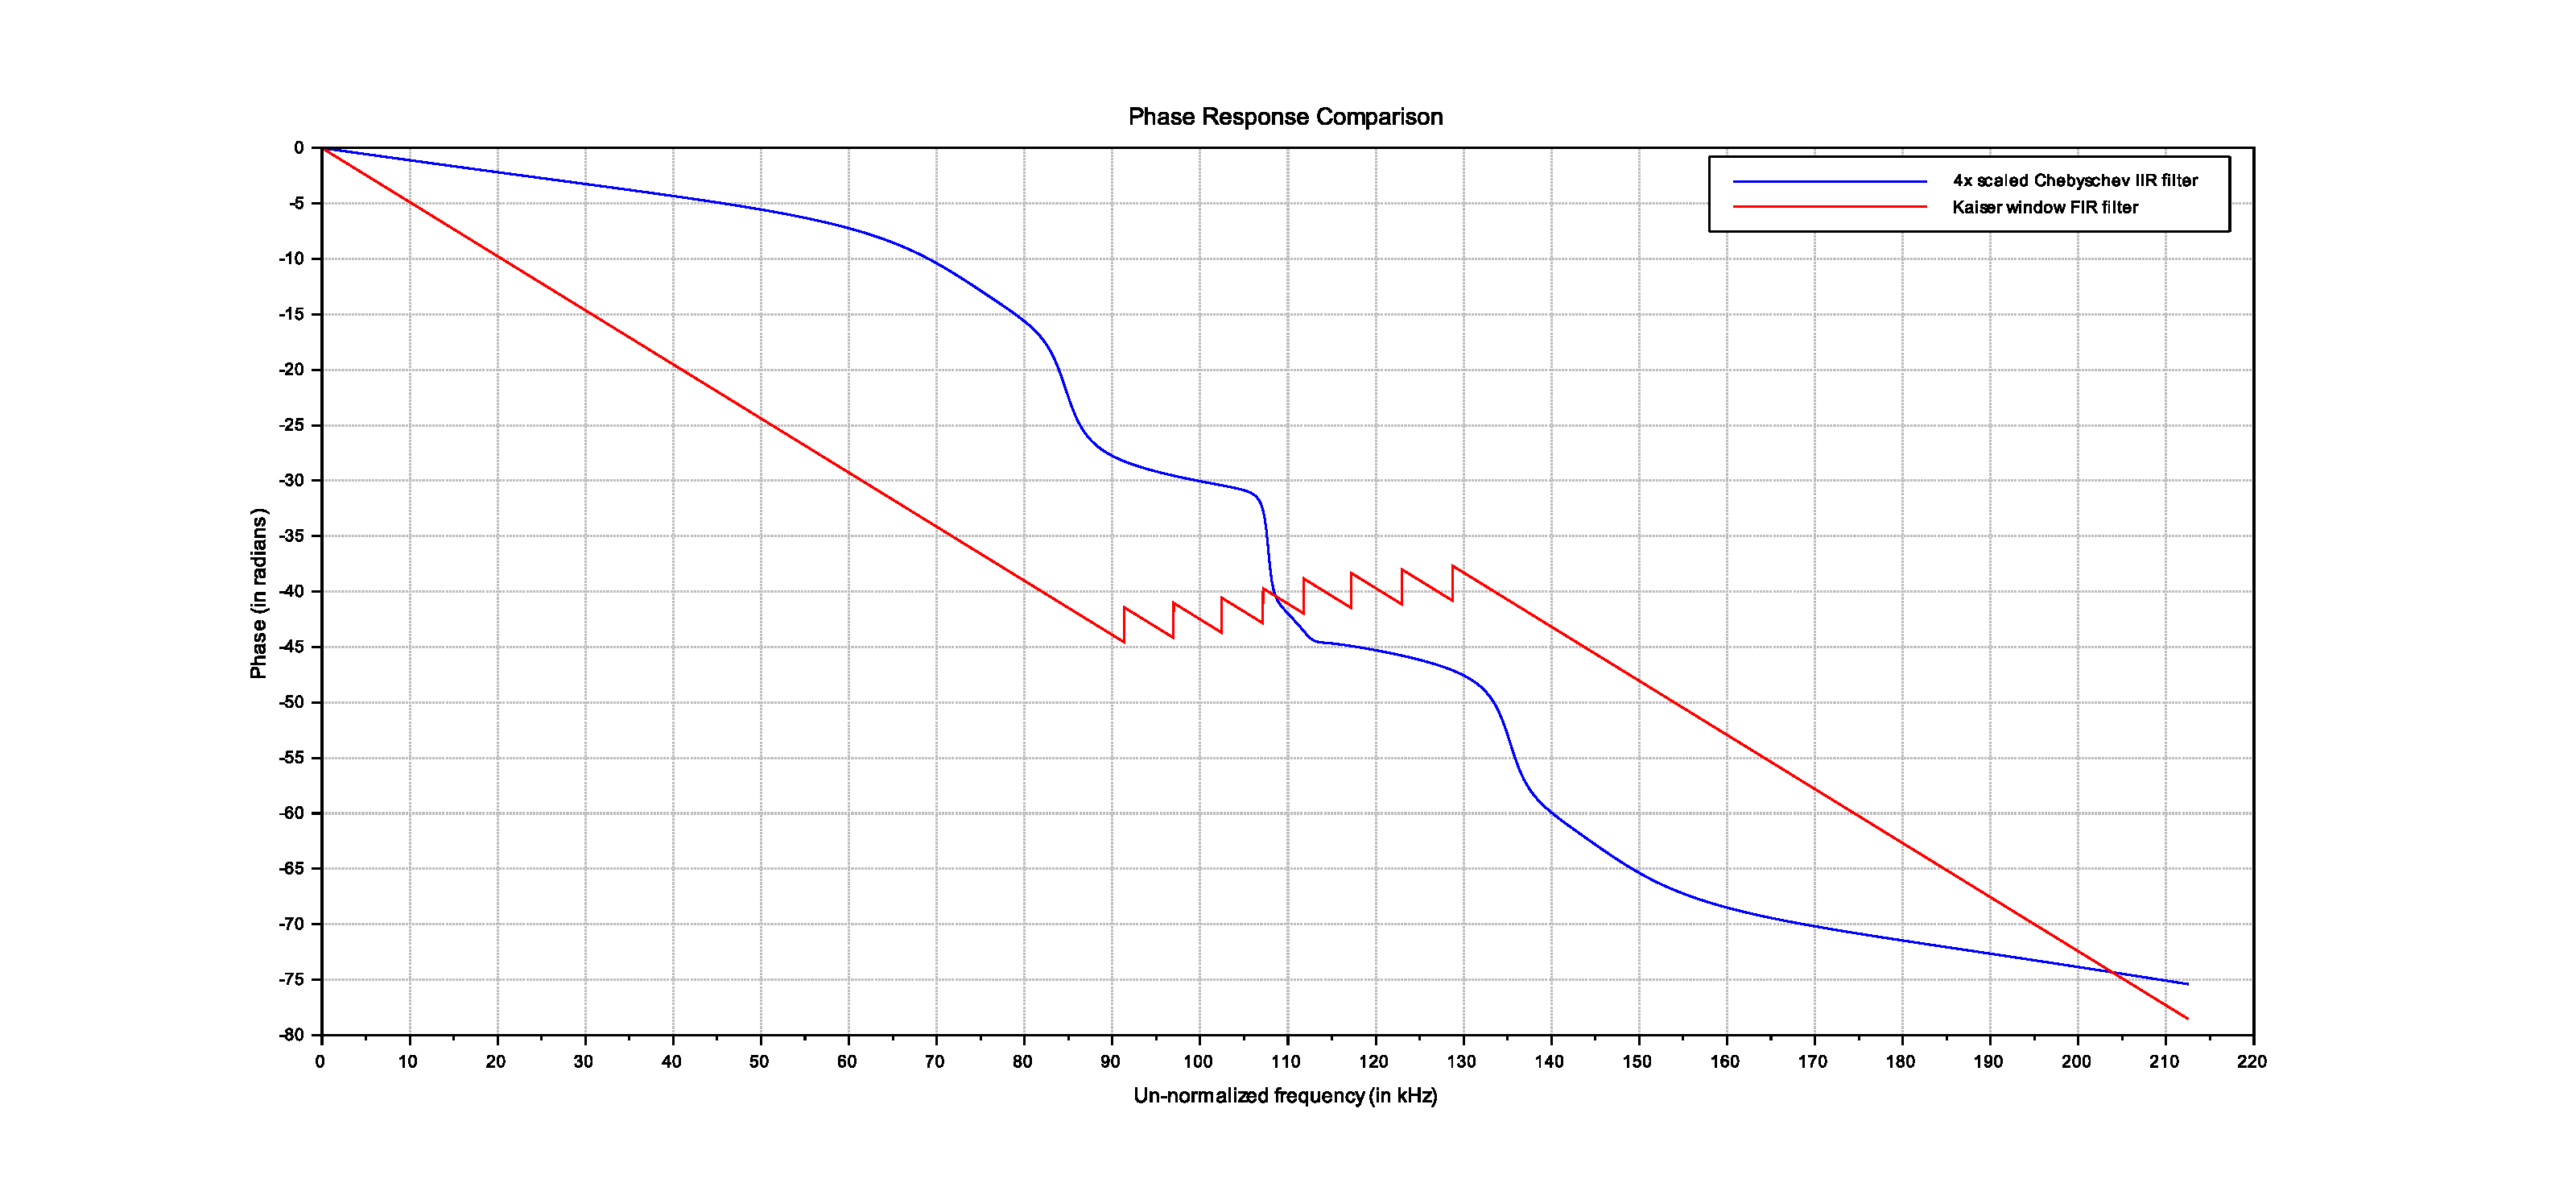
\includegraphics[width=1.5\textwidth]{comp_bs_phase.pdf}}
\end{figure}

\end{document}
